Hier wird auf die Änderungen der Performanz der Netze eingegangen, die dadurch entstehen, wenn der Targetdatensatz unterschiedliche Größen hat. 
Die Vermutung ist, dass es schlechter wird, je weniger Daten vorhanden sind. 

Um Vergleiche zu haben, die zueinander passen, werden wieder insgesamt 40 Epochen trainiert und nach zwanzig TF vollzogen. Dies wird mit den 
Netzwerken 
CMP, 1DC und COD durchgeführt. Hier wird auch auf den Testdatensatz eingegangen. 

\begin{figure}[htpb]
    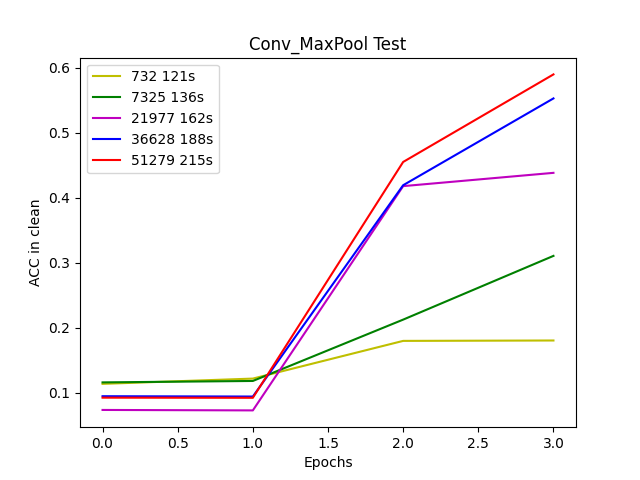
\includegraphics[height=5cm]{../../Plots/ba_plots/targetgroesse/cmp_ts.png}
    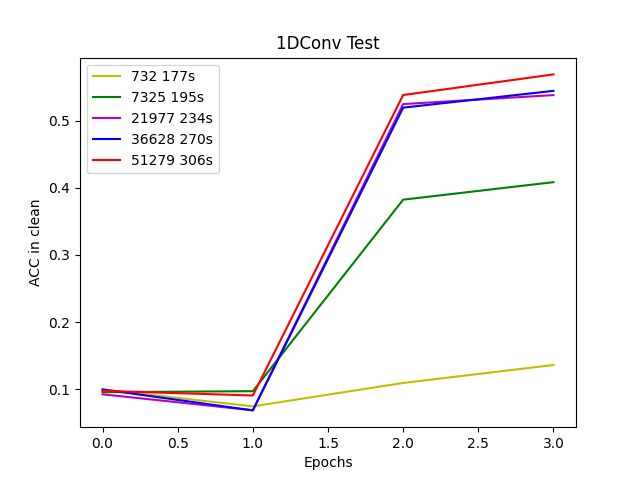
\includegraphics[height=5cm]{../../Plots/ba_plots/targetgroesse/1dc_ts.png}
    \caption{\label{fig:targetgroessedeepdir} 
    \small{Hier ist die Veränderung der Accuracy bei Convolution Netzen zu sehen, wenn die Größe des Targetdatensatzes verändert wird. 
    Es sind jeweils die Plots über die Testdaten des Targetdatensatzes, wobei links CMP und rechts 1DC ist. 
    Dahinter sind folgende Tests: CMP: und 
    1DC:TF2/732/10, 1DC:TF2/7k/10, 1DC:TF2/21k/10, 1DC:TF2/36k/10, 1DC:TF2/51k/10 jeweils in den Farben gelb, grün, lila, blau und rot. 
    }}
\end{figure}

In Figure 4.1 sieht man die Testdatenläufe bezüglich der Menge der Trainingsdaten. Dabei ist die erste Zahl in der Legende die Menge und die 
Zweite die Dauer. Dabei bezieht die Menge sich nur auf den Targetdatensatz. Es wird deutlich, dass es länger dauert, je mehr Daten vorhanden sind. 
Ebenso bestätigt sich die Vermutung, dass es auch bei Kaskadennetzwerken mit TF besser wird, je mehr Daten vorhanden sind. 
Ebenfalls zeigt sich, dass Deep Cascade etwas besser ist als Direct Cascade. Dies dürfte daran liegen, dass Direct Cascade Netzwerke sind, 
die nur ein Hidden Layer haben, während es bei Deep Cascade mehrere sind. 

\begin{figure}[htpb]
    \centering
    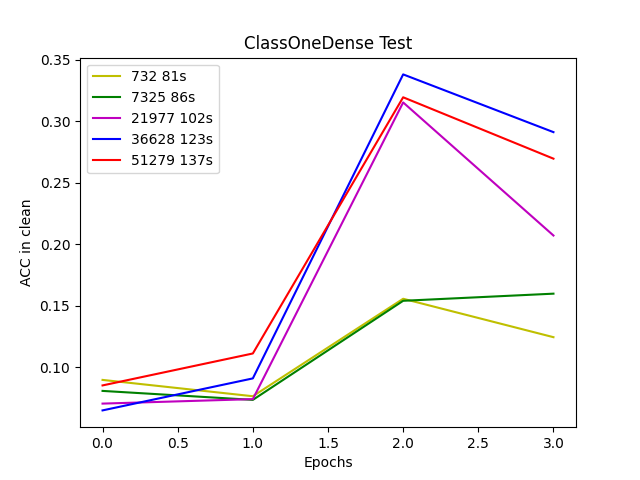
\includegraphics[height=5cm]{../../Plots/ba_plots/targetgroesse/cod_ts.png}
    \caption{\label{fig:targetgroesselinear} 
    \small{Hier ist die Veränderung der Test-Accuracy bei Linearen Netzwerk zu sehen, wenn die Größe des Targetdatensatzes verändert wird. 
    Es sind die Tests COD:TF2/732/10, COD:TF2/7k/10, COD:TF2/21k/10, COD:TF2/36k/10 und COD:TF2/51k/10 in den Farben gelb, grün, lila, blau und 
    rot. }}
\end{figure}

In Figure 4.2 ist das Deep Cascade Netzwerk, welches als Hidden Layer ausschließlich Linearlayer hat. Auffällig ist, dass dieses bei egal 
wievielen Datensamples immer schlechter abschneidet als die anderen beiden Netzwerke, die Convolutionlayer besitzen. 
Dies liegt daran, dass dieses Netzwerk die wichtigen Bilderkennungsfeatures nicht ausreichend herausfiltern kann, weil die Daten zu komplex und 
nicht linear sind. 

Generell ist es bei allen Testplots so, dass sie nie eine annehmbar hohe Accuracy besitzen und das auch dann nicht, wenn es genügend Daten 
gibt, damit auf dem Targetdatensatz direkt gelernt werden könnte. Wenn dies mit dem Deep Cascade Netzwerk gemacht wird, kommt dabei eine 
Accuracy von etwa 70\% heraus, was deutlich besser als jedes TF Netzwerk ist. 
